\documentclass[11pt]{article}

%packages
\usepackage{graphicx}
\usepackage{fullpage}
\usepackage{amsmath}
\usepackage{amssymb}
\usepackage[pdfborder={0,0,0}]{hyperref}
\usepackage{pdfpages}
\usepackage[parfill]{parskip}
\usepackage{wrapfig}

% title
%\author{Andy Barry}
%\title{}

\begin{document}

%\maketitle

{\LARGE National University of Malaysia / UTM Helicopter Workshop}
\hrule

\section*{Main Objectives}

\begin{itemize}
    \item Develop teamwork skills by simultaneously building hardware and software with a group of four people
    \item Get past barriers such as, ``I can’t build electronics," ``I don’t know enough to write a computer program," ``I'm not smart enough to do engineering."
    \item Learn problem-solving skills that work in a wide variety of math, science, and engineering situations.
    \item Understand the full process for building and programming a useful microelectronics system.
    \item Build debugging skills for identifying, understanding, and solving common problems in these types of systems
    \item Learn to program a microprocessor
    \item Complete and fly an autonomous flight system
    \item Show that learning can be fun; inspire students to learn more on their own and take the skills learned in the workshop to higher levels.
\end{itemize}

\section*{Executive Summary}
\begin{wrapfigure}{r}{0.5\textwidth}
  \begin{center}
    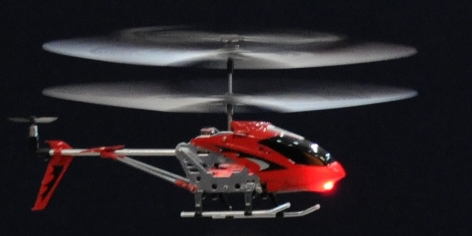
\includegraphics[width=0.48\textwidth]{figures/S107G.jpg}
    \caption{S107G micro-helicopter. Image courtesy of FIAP.}
  \end{center}
\end{wrapfigure}
Students work in small teams of approximately four members.  Each team has a computer, breadboard, microprocessor, visible LED light, infrared LED light array, battery pack, amplifier, and small helicopter.  Students start by building a simple circuit that blinks the visible LED to familiarize themselves with the different components and how to program the microprocessor.

Once the students are accustomed to their components and environment, we guide them through the process of building a more complicated circuit that uses an amplifier to power the LED array while explaining why the microprocessor alone is unable to provide enough energy.  As they are working on their circuits, the students learn debugging techniques, such as blinking LEDs at important points in the software and utilizing a mobile phone camera to detect infrared light.

With the circuits built and tested, the workshop transitions to discussing control systems and autonomous robotics.  Each team loads software onto their microprocessor that issues commands to their helicopters (via the IR LED array circuit they just built), but is not programmed for flight maneuvers.  The teams fly the helicopters through this interface and gain a complete understanding on the variables required for success.  We then challenge them to perform a specific autonomous maneuver with the helicopters, such as a takeoff, mid-air box, and landing.

As teams program their systems to fly, incrementally succeeding at each step (takeoff, landing, turning, flying straight), we work with them individually to help them debug the systems and interpret the systems’ outputs, especially when they are unexpected.

For a final demonstration of the techniques, each team chooses a more complicated maneuver to fly and programs their system to perform that operation.  During this period, we discuss how feedback could make these systems better, and discuss common ways to implement feedback loops.

The workshop closes with a summary of the vast amount of material covered and a short discussion of how these techniques are applicable to many other systems beyond flight control.

\section*{Workshop in Detail}
% In just four hour students learn to build circuits, program microprocessors, and write open-loop control software for micro helicopters.
\subsection*{Step 1: Build a Circuit}
\begin{wrapfigure}{r}{0.4\textwidth}
    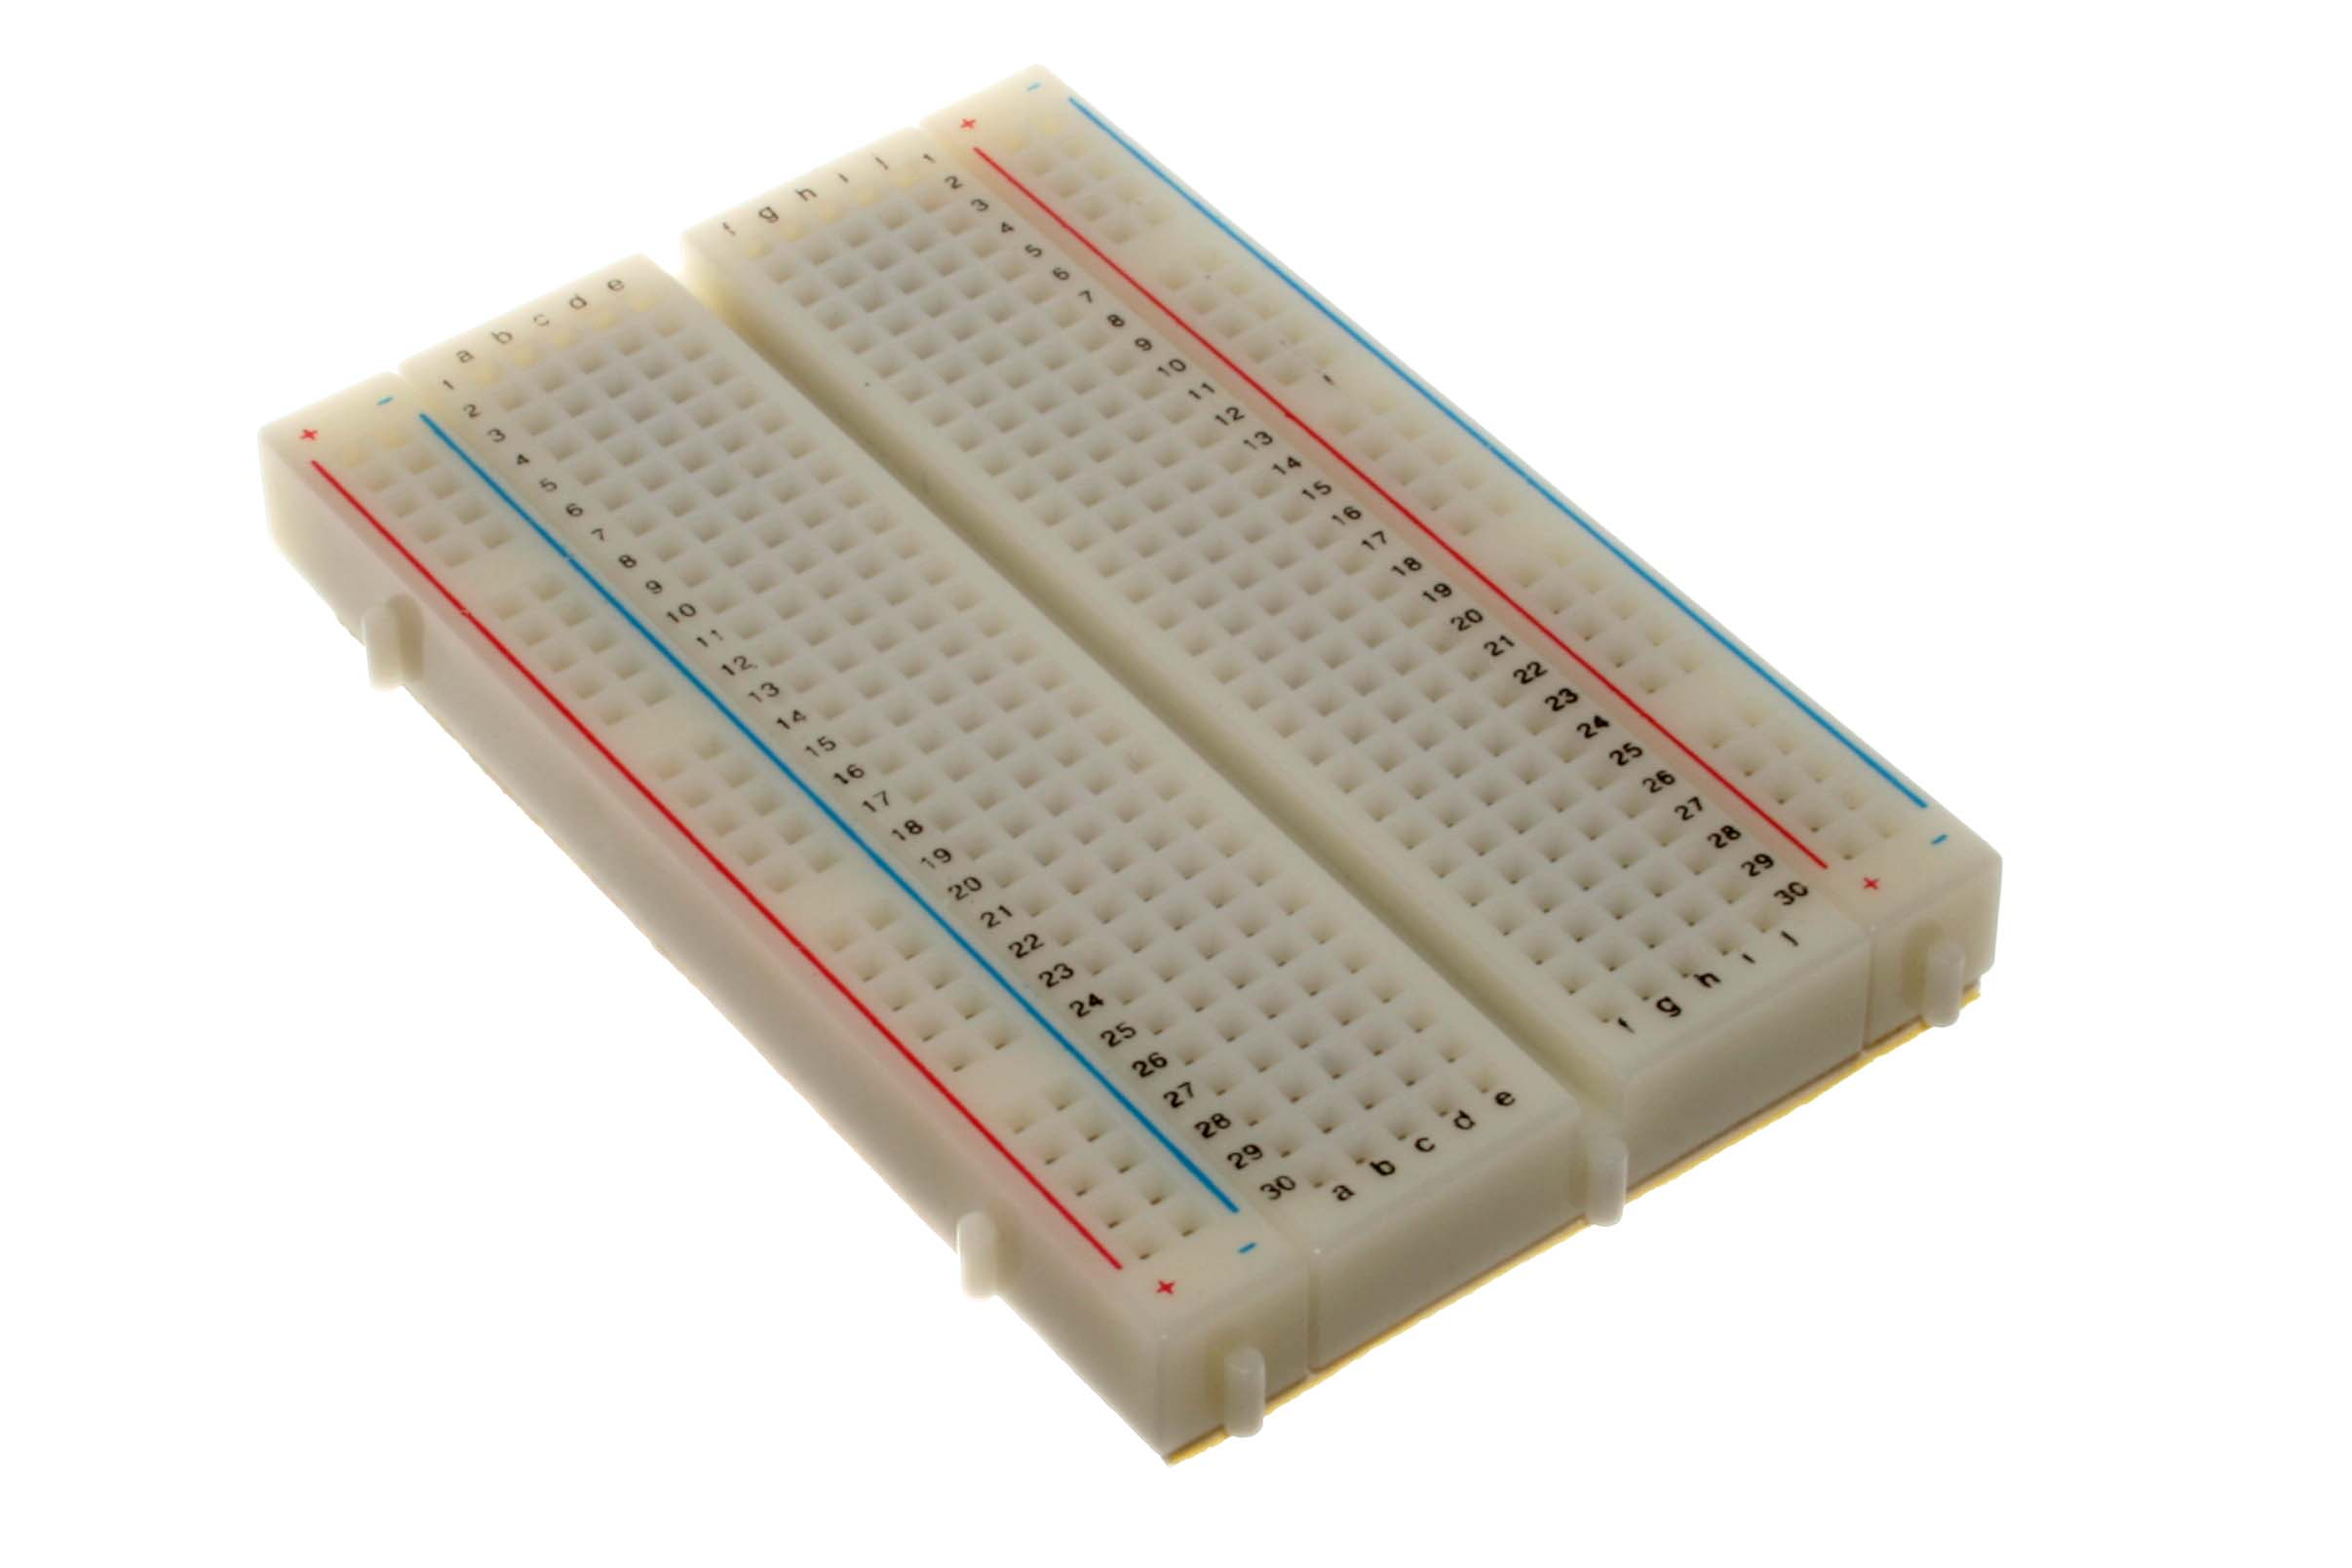
\includegraphics[width=0.38\textwidth]{figures/400_points_breadboard.jpg}
    \caption{\label{breadboard}
        A breadboard. Image courtesy of Oomout Ltd.
    }
\end{wrapfigure}
Assuming no prior knowledge of circuit design or construction, we instruct students on circuit design and construction.  Starting with how to use a breadboard (Figure \ref{breadboard}), and move on to the basic use of a mircoprocessor.  Each group builds a simple circuit and programs their microprocessor to blink a light.




%\begin{thebibliography}{1}

%\bibitem{bookName}
% Book

%\end{thebibliography}

%\begin{figure}
%\includegraphics[width=\textwidth]{}
%\caption{
%    Caption
%    \label{fig}
%}
%\end{figure}

%\includepdf[pages=-]{}

%\begin{table}
%\begin{tabular}{|r|r|}
%\hline
%Col Header 1&Col Header 2\\
%\hline
%4&18\\
%5&24\\
%6&22\\
%7&35\\
%\hline
%\end{tabular}
%\caption{
%    Table
%    \label{table}
%}
%\end{table}

\end{document}

